%!TEX TS-program = pdflatex
%!TEX encoding = UTF-8 Unicode

\documentclass[11pt]{article}

\usepackage[utf8]{inputenc}
\usepackage{geometry}
\geometry{a4paper}
\usepackage{graphicx}
\usepackage{booktabs}
\usepackage{array}
\usepackage{verbatim}
\usepackage{subfig}
\usepackage{hyperref}

\usepackage{fancyhdr} 
\pagestyle{fancy}
\renewcommand{\headrulewidth}{0pt} 
\lhead{}\chead{}\rhead{}
\lfoot{}\cfoot{\thepage}\rfoot{}

\usepackage{sectsty}
\allsectionsfont{\sffamily\mdseries\upshape}

\usepackage[nottoc,notlof,notlot]{tocbibind} 
\usepackage[titles,subfigure]{tocloft} 
\renewcommand{\cftsecfont}{\rmfamily\mdseries\upshape}
\renewcommand{\cftsecpagefont}{\rmfamily\mdseries\upshape}

\usepackage[spanish]{babel}
\usepackage{listings}

%%%El documento comienza aqui

\title{\textbf{Investigacion de Lenguajes - Smalltalk}}
\author{\textbf{Jimmy Banchon - Rene Balda}}
\date{\textbf{\today}}
\begin{document}
\maketitle
\section{\textbf{Introducción}} 
\paragraph{} \noindent
Smalltalk es un lenguaje de programación orientada a objeto puro, se basa en la comunicación entre objetos mediante envio de mensajes, está considerado como el primer lenguaje de este paradigma, ya que  en \textbf{Smalltalk} todo es un objeto; éste influyo drásticamente en el surgimiente de lenguajes como JAVA, PHP, Python, Ruby y muchos de los actuales lenguajes orientados a objetos.
 \textbf{Smalltalk} es mucho mas que un lenguaje de programación, es un ambiente completo de desarrollo de programas,que integra muchas caracteristicas, que lo hacen un sistema de ventanas y manejador de codigo fuente.
\section{\textbf{Características}}
Las principales características de  \textbf{Smalltalk} son:
\subsection{\textbf{Orientado a Objetos:}}
\textbf{Smalltalk} por ser un lenguaje de programacion orientado a objeto puro, en el todo tipo de dato es una instancia de una clase, es por eso, que la comunicacion entre objetos se hace por envio de mensajes.
\subsection{\textbf{Tipado Dinamico:}}
En \textbf{Smalltalk} una variable puede tomar valores de distinto tipo en distintos momentos.
\ subsection{\textbf{Compilacion JIT}}
\textbf{Smalltalk} es un lenguaje interpretado, es decir, el codigo fuente es traducido a bytecode para que luego este sea traducido a lenguaje de maquina, esta caracteristica hace que el programa compilado sea multiplataforma y compatible con cualquier arquitectura.
\ subsection{\textbf{Garbage Collection:}}
\textbf{Smalltalk} utiliza este mecanismo de gestion de memoria, para que el usuario no deba hacer una subrutina para liberar memoria cuando no hayan objetos referenciados a alguna variable.
\section{Historia}
\paragraph{} \noindent
EL comienzo de lo que se conocería como programación orientada a objeto tuvo sus origines en Simula-67 pero luego el desarrollo fue completado con la evolución del lenguaje \textbf{Smalltalk}.
\paragraph{} \noindent
Para este paradigma la implementación y la definición estructural de los procesos se ocultó de las unidades del programa que las usan, este paradigma fue popular en los 1980s.
\paragraph{} \noindent
El principal responsable del desarrollo fue Alan Kay, entre sus principales logros fue darle mayor interactividad y uso de gráficos en los programas para que el usuario obtenga una interfaz mucho más amigable de lo que se mostraba en ese entonces.
\paragraph{} \noindent
El lenguaje de programación FLEX todavía estaba muy orientado a los especialistas, por lo que Kay decidió tomar algunas ideas de LOGO para hacerlo más fácil de usar. Así nació Smalltalk[1].
\paragraph{} \noindent
Este a su vez fue implementado en el modelo Alto salido de Xerox PARC. La primera versión fue smalltalk-80, anterior a esta fue creada smalltalk-71 desarrollada por Dan Ingallis que dio a conocer un lenguaje de programación que se podía reducir a una página de código. Pero esta version fue bastante diferente de lo que sería la que conocemos.
\paragraph{} \noindent
Los sistemas operativos orientados a objetos de Apple Computers fueron inspirados por \textbf{Smalltalk}.
\section{Tutorial de Instalación}
\paragraph{} \noindent
Para comenzar a programar en smalltalk nos descargaremos Squeak el cual es una implementación de smalltalk este es el link \href{http://www.squeak.org/Download/}{Squeak All in one}
Al abrir la página nuestro link de descarga se encontrara en donde nos dice la figura siguiente.

				\begin{center}
				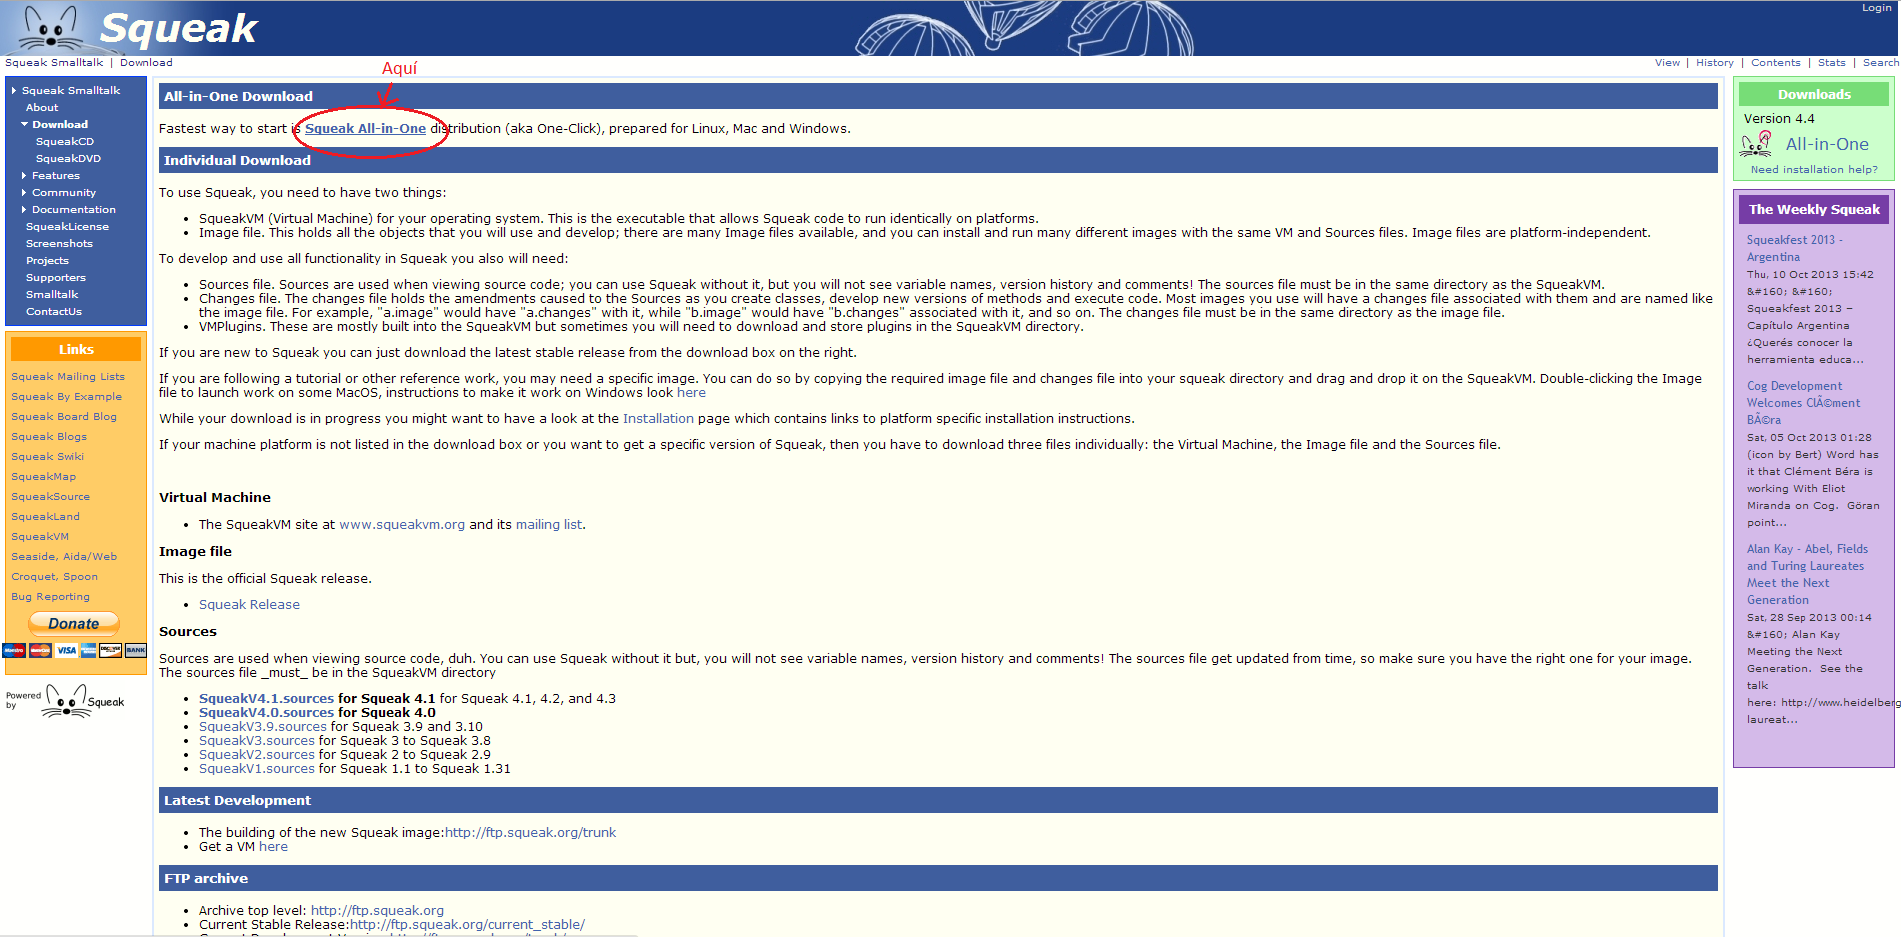
\includegraphics[width=0.8\textwidth]{./tutorial}
				\end{center}
\paragraph{} \noindent
Una vez descargado lo descomprimimos en una carpeta y dentro encontraremos el ejecutable de Squeak para de aqui realizar nuestro primer programa en este lenguaje.

				\begin{center}
				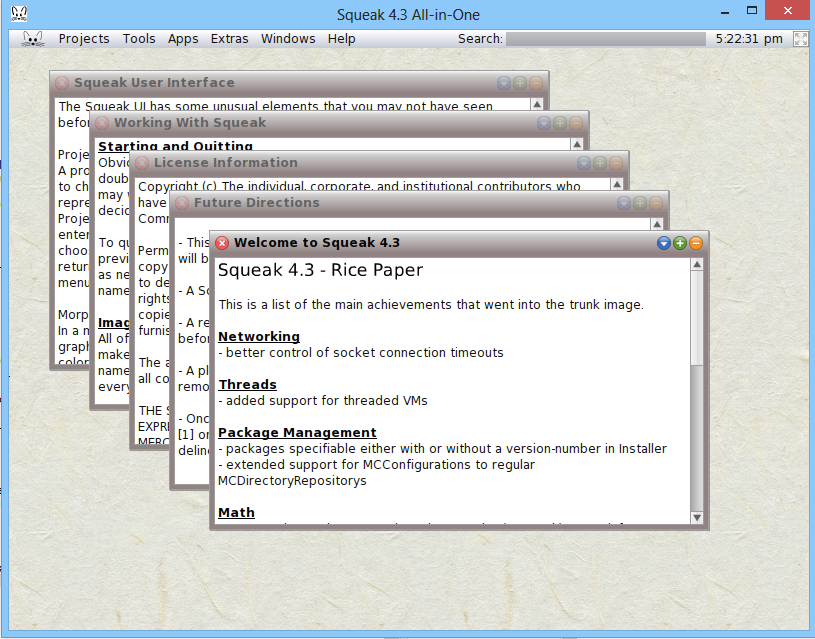
\includegraphics[width=0.8\textwidth]{./squeak}
				\end{center}

\section{Hola Mundo y otros Programas Introductorios}
\section{Referencias}
\begin{enumerate}
	\item \href{http://computacion.cs.cinvestav.mx/~acaceres/courses/itesm/lp/clases/lp12.pdf}{http://computacion.cs.cinvestav.mx/~acaceres/courses/itesm/lp/clases/lp12.pdf}
\end{enumerate}

\end{document}